\chapter{Specifications}\label{specifications}

\section{Functional Description}\label{functional-description}

The Roa Logic AHB-Lite Multi-layer Interconnect is a highly configurable
interconnect fabric for AMBA AHB-Lite based systems, enabling multiple
masters to be connected to multiple slaves.

Connections are dynamically created based on which slave a master is
addressing, and once created enable direct communication between master
and slave without other masters being aware or interfering.

A new connection is typically created within one clock cycle, providing
high bandwidth and low latency communication between master and slave.

\begin{figure}[tbh]
	\centering
	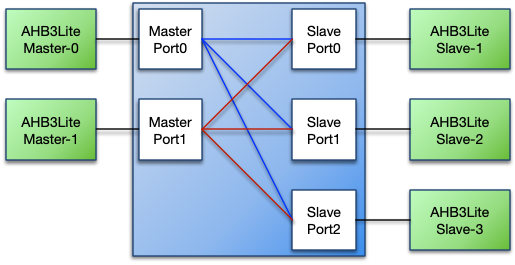
\includegraphics{assets/img/ahb-lite-switch-sys1}
	\caption{Example Master / Slave Communication Setup}
	\label{fig:ahb-lite-switch-sys1}
\end{figure}

\section{Master Port}\label{master-port}

An AHB-Lite bus master connects to a master port of the Multi-layer
Interconnect. The master port is implemented as a regular AHB-Lite slave
interface thereby allowing support for complex bus structures.

The following figure shows an example bus structure where a bus master -- Master-1
-- has two directly connected slaves; the Interconnect-Master-Port1 and
Slave-4

\begin{figure}[tbh]
	\centering
	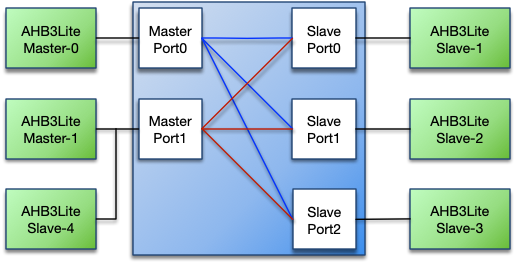
\includegraphics{assets/img/ahb-lite-switch-sys2}
	\caption{Connectivity Example for 2 Bus Masters, 4 Slaves}
	\label{fig:ahb-lite-switch-sys2}
\end{figure}

To access a slave, the Interconnect first checks if the designated slave
port is available. If it is available the slave port immediately
switches to the requesting master. If the slave port is occupied due to
another master accessing the slave, the master port generates wait
states until the requested slave becomes available. Note the pipelined
nature of the AHB-Lite bus may cause a single wait state to be inserted
when the slave switches to a new master.

The slave port always retains the connection to the master until another
master requests access to that slave port; this enables the original
master to request further access to the slave without incurring any
delay due to arbitration.

\subsection{Master Priority}\label{master-priority}

Each master port has a priority level port (\texttt{mst\_priority[]}).

When multiple masters with different priority levels request access to
the same slave port, access is always granted to the master with the
highest priority level. If a new master requests access while a
transaction is already in progress, access will be granted according to
its priority, ahead of any waiting lower priority masters. If masters
have the same priority level, then access is granted based on a
round-robin scheme.

Master priority may be set dynamically, however assigning a static
priority results in a smaller Interconnect and reduces timing paths. The
priority value may only be changed while the master port is idle; i.e.
\texttt{mst\_HSEL} is negated (`0') and/or when \texttt{mst\_HTRANS} is IDLE.

\subsection{Bus Locking Support}\label{bus-locking-support}

The priority levels determine the order in which masters are granted
access to the slave port. The slave port switches between masters when
the current accessing master is idle (\texttt{mst\_HSEL} is negated and/or
\texttt{mst\_HTRANS} = IDLE) or when the current burst completes.

However the current master may lock the bus by asserting \texttt{HMASTLOCK}; this
prevents the slave port switching.

\subsection{Specifying the number of Master
Ports}\label{specifying-the-number-of-master-ports}

The number of master ports is specified by the \texttt{MASTERS} parameter.

\section{Slave Port}\label{slave-port}

An AHB-Lite bus slave connects to a slave port of the Multi-layer
Interconnect. The slave port is implemented as a regular AHB3-Lite master
interface thereby allowing support for complex bus structures such as
shown below:

\begin{figure}[tbh]
	\centering
	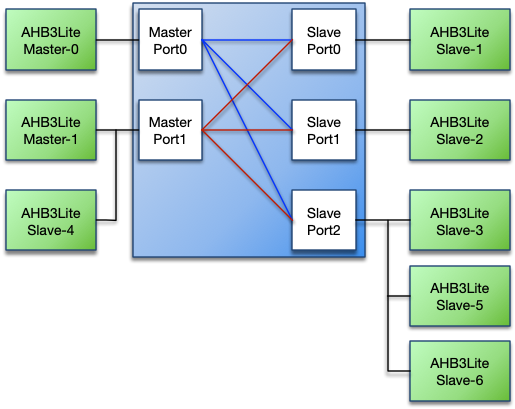
\includegraphics{assets/img/ahb-lite-switch-sys3}
	\caption{Connectivity Example	for 2 Bus Masters, 6 Slaves}
	\label{fig:ahb-lite-switch-sys3}
\end{figure}

\subsection{Address Space
Configuration}\label{address-space-configuration}

Each slave port has an address base (\texttt{slv\_addr\_base}) and address mask
(\texttt{slv\_addr\_mask}) port. Together these set the address range covered by
the slave port.

The address base port specifies the base address for the address range
covered by the slave port and the address mask port defines the address
range covered by the slave port. The internal port select signal is
specified as \texttt{slv\_addr\_base} AND \texttt{slv\_addr\_mask}.

The address base and address mask values may be changed dynamically,
however assigning static values results in a smaller Interconnect and
reduces timing paths. Address base and address mask may only be changed
when the slave port(s) are idle. Since multiple masters may be active at
the same time trying to access the interconnect, special care must be
taken to ensure no master accesses the Interconnect while updating the
address base and address mask values.

The slave port asserts \texttt{HSEL} when accesses are within the port's address
range. When the port is not being accessed \texttt{HSEL} is negated (`0'), but
\texttt{HTRANS} and other AMBA signals will still provide data. These signals
must be ignored while \texttt{HSEL} is negated (`0').

The slave port will output the full address, i.e. all \texttt{HADDR\_SIZE} bits,
on its address bus (\texttt{slv\_HADDR}). Connected AMBA slaves should use the
relevant least significant bits (LSBs) only.

\pagebreak

\subsubsection{Example 1}\label{example-1}

\begin{verbatim}
slave_addr_base = 32'h1000_0000
slave_addr_mask = 32'hF000_0000
Address-range = 32'h1000_0000 to 32'h1FFF_FFFF
\end{verbatim}

\subsubsection{Example 2}\label{example-2}

\begin{verbatim}
slave_addr_base = 32'h4000_0000
slave_addr_mask = 32'hE000_0000
Address-range = 32'h4000_0000 to 32'h5FFF_FFFF
\end{verbatim}

\subsection{Slave Port HREADYOUT and HREADY
Routing}\label{slave-port-hreadyout-and-hready-routing}

The slave port has an \texttt{HREADYOUT} port, which is not part of the AHB-Lite
specification. It is required to support slaves on the master's local
bus. The \texttt{HREADY} signal, generated by the multiplexor, is driven to the
addressed slave's \texttt{HREADYOUT} port.

\begin{figure}[thb]
	\centering
	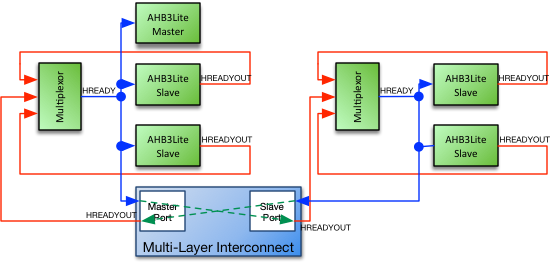
\includegraphics[]{assets/img/ahb-lite-switch-sys4}
	\caption{HREADYOUT and HREADY Routing}
	\label{fig:hready-hready-routing}
\end{figure}

The simple case of where only one master is connected to a master port
or where only a single slave is connected to a slave port is illustrated
below.

There are no multiplexors on either the master bus or the slave bus.
Since there is no other slave on the master bus, its \texttt{HREADY} signal is
only driven by the master port's \texttt{HREADYOUT} signal. Thus the master
port's \texttt{HREADYOUT} drives both the master's \texttt{HREADY} input and the master
port's \texttt{HREADY} input.

Similarly since there is no other slave on the slave bus, the slave
port's \texttt{HREADYOUT} signals drives the slave's \texttt{HREADY} input and the slave's
\texttt{HREADYOUT} signal drives the slave port's \texttt{HREADY} input.

\begin{figure}[htb]
	\centering
	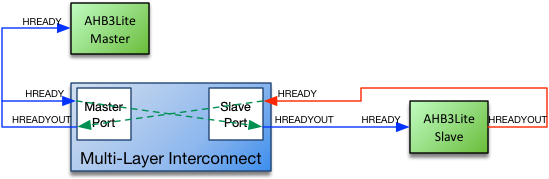
\includegraphics{assets/img/ahb-lite-switch-sys5}
	\caption{Single Master/Slave Routing}
	\label{fig:master-slave-routing}
\end{figure}

% Avoid previous figure being isolated on page
\newpage

\subsection{Specifying the number of Slave
Ports}\label{specifying-the-number-of-slave-ports}

The number of slave ports is specified by the \texttt{SLAVES} parameter.
